\chapter{Campo de los números complejos}

\section{Definiciones y propiedades algebraicas}

\begin{defi}
El \textbf{sistema de los números complejos}, denotado por $\mathbb{C}$, es el conjunto $\mathbb{R}^2$ junto con las operaciones:

\begin{enumerate}
\item de adición
\begin{equation}
(x_1, y_1) + (x_2,y_2) = (x_1 + y_1, x_2 + y_2) \label{Suma}
\end{equation}

\item y de multiplicación compleja siguiente:
\begin{equation}
(x_1, y_1) (x_2,y_2) = (x_1 x_2 - y_1y_2, x_1 y_2 + y_1x_2). \label{Multiplicacion}
\end{equation}

\end{enumerate}

Los elementos $z = (x,y)$ de $\mathbb{C}$ se llaman \textbf{números complejos}, donde $x$ es la \textbf{parte real} de $z$ e $y$ la \textbf{parte imaginaria}. Lo anterior se denota por
$$Re(z) = x ~~\mbox{e}~~ Im(z) = y.$$

Diremos que un complejo es \textbf{imaginario puro} si $z = (0,y)$. En particular, al número $(0,1)$ lo denotaremos por $i$.
\end{defi}

\textbf{Observación:} Cada número real $x$ puede ser identificado como el complejo $z = (x,0)$; de esta manera, asumiremos siempre que $\mathbb{R} \subset \mathbb{C}$. Notar que si $z_1 = (x_1,0)$ y $z_2 = (x_2,0)$, entonces
\begin{eqnarray*}
z_1 + z_2 &=& (x_1 + x_2, 0), \\
z_1z_2 &=& (x_1x_2, 0),
\end{eqnarray*}

es decir, que las operaciones \eqref{Suma} y \eqref{Multiplicacion} coinciden con las operaciones en $\mathbb{R}$. Más aún, si $(\alpha,0) \in \mathbb{R}$ y $z = (x,y)$ es cualquier otro complejo, se tiene
$$(\alpha,0)z = (\alpha x, \alpha y),$$

es decir, tenemos la operación multiplicación por escalar en $\mathbb{R}^2$.

\begin{defi}
Diremos que dos complejos $z_1 = (x_1,y_1)$ y $z_2 = (x_2, y_2)$ son iguales si y sólo si
$$x_1 = x_2 ~\wedge~ y_1 = y_2.$$
\end{defi}

En lugar de usar $(x,y)$  para representar a los números complejos, encontraremos otra forma más conveniente y natural de identificarlos. 
Si $z = (x,y) \in \mathbb{C}$, entonces
\begin{eqnarray*}
z &=& (x,y) \\
&=& (x,0) + (0,y) \\
&=& (x,0) + (y,0) (0,1) \\
&=& x + yi = x+iy.
\end{eqnarray*}

Esta forma de denotar a los números complejos es conocida como \textbf{forma binómica} de $z$.

\begin{teorema}
El conjunto $\mathbb{C}$ con las operaciones \eqref{Suma} y \eqref{Multiplicacion} resulta ser un cuerpo conmutativo.
\end{teorema}

\begin{proof}
Sean $z_1 = (x_1,y_1)$, $z_2 = (x_2,y_2)$ y $z_3 = (x_3, y_3)$ números complejos cualesquiera. Probaremos los 9 axiomas de los cuerpos conmutativos, teniendo en cuenta que $\mathbb{R}$ es un cuerpo. 

\begin{enumerate}
\item La suma es conmutativa. En efecto,
$$z_1 + z_2 = (x_1 + x_2, y_1 + y_2) = (x_2 + x_1, y_2 + y_1) = z_2 + z_1.$$

\item La suma es asociativa. En efecto,
\begin{eqnarray*}
z_1 + (z_2 + z_3) &=& (x_1,y_1) + ((x_2,y_2) + (x_3,y_3)) \\
&=& (x_1 ,y_1) + (x_2 + x_3, y_2 + y_3 )  \\
&=& (x_1 + (x_2 + x_3), y_1 + (y_2 + y_3)) \\
&=& ((x_1 + x_2) + x_3, (y_1 + y_2) + y_3) \\
&=& (x_1 + x_2, y_1 + y_2)  + z_3 \\
&=& (z_1 + z_2) + z_3.
\end{eqnarray*}

\item Existe un elemento neutro para la suma. En efecto, si consideramos el complejo $(0,0)$, se tiene
$$z_1 + (0,0) = (x_1,y_1) + (0,0) = (x_1, y_1) = z_1.$$

\item Cada $z_1$ tiene un inverso para la suma. En efecto, si consideramos el complejo $(-x_1, -y_1)$, se verifica
$$z_1 + (-x_1, -y_1) = (x_1 + (-x_1), y_1 + (-y_1)) = (0,0).$$

\item El producto es conmutativo. En efecto, 
$$z_1 z_2 = (x_1, y_1) (x_2,y_2) = (x_1 x_2 - y_1y_2, x_1 y_2 + y_1x_2) = (x_2 x_1 - y_2y_1,  x_2y_1 + y_2x_1 ) = z_2 z_1.$$

\item El producto es asociativo. En efecto,
\begin{eqnarray*}
z_1 (z_2 z_3) &=& (x_1,y_1) (x_2x_3 - y_2y_3, x_2y_3 + y_2 x_3) \\
&=& (x_1(x_2 x_3 - y_2y_3) - y_1 (x_2y_3 + y_2 x_3), x_1 (x_2y_3 + y_2x_3) + y_1(x_2x_3 - y_2y_3)) \\
&=& ((x_1x_2 - y_1y_2)x_3 - (x_1 y_2 + y_1x_2)y_3 , (x_1 x_2 - y_1y_2) y_3 + (x_1 y_2 + y_1 x_2)x_3) \\
&=& (x_1 x_2 - y_1y_2, x_1y_2 + y_1 x_2)(x_3,y_3) \\
&=& (z_1 z_2) z_3.
\end{eqnarray*}

\item Existe un elemento neutro para el producto. En efecto, si consideramos el complejo $(1,0)$, se tiene
$$z_1 (1,0) = (x_1 - 0, 0 + y_1) = (x_1,y_1) = z_1.$$

\item Cada $z_1 \neq (0,0)$ tiene un inverso para el producto. En efecto, supongamos que existe $w = (w_x, w_y) \in \mathbb{C} \setminus \{(0,0)\}$ tal que
$$z_1 w = (1,0) ~\Leftrightarrow~(x_1 w_x - y_1 w_y, x_1w_y + y_1 w_x) = (1,0).$$

Por igualdad de los números complejos:
\begin{equation*}
 \left\{ \begin{array}{ccl}
x_1 w_x - y_1 w_y &=& 1 \\
y_1 w_x + x_1 w_y &=& 0
\end{array}  \right.  ~\Leftrightarrow~ \left\{ \begin{array}{ccl}
 w_x  &=& \frac{x_1}{x_1^2 + y_1^2} \\
 w_y &=& - \frac{y_1}{x_1^2 + y_1^2}
\end{array}  \right.  .
\end{equation*}

Como $z_1 \neq (0,0)$, $w$ está bien definido y por las equivalencias hemos probado que existe el inverso multiplicativo.

\item El producto es distributivo con respecto a la suma. En efecto,
\begin{eqnarray*}
z_1 (z_2 + z_3) &=& (x_1, y_1) (x_2 + x_3, y_2 + y_3) \\
&=& (x_1 (x_2 + x_3) - y_1(y_2 + y_3), x_1 (y_2 + y_3) + y_1(x_2 + x_3)) \\
&=& ((x_1x_2 - y_1 y_2) + (x_1x_3 - y_1y_3), (x_1 y_2 + y_1 x_2) + (x_1 y_3 + y_1 x_3)) \\
&=& (x_1 x_2 - y_1 y_2, x_1 y_2 + y_1x_2) + (x_1 x_3 - y_1y_3, x_1 y_3 + y_1 x_3) \\
&=& z_1 z_2 + z_1 z_3.
\end{eqnarray*}
\end{enumerate}

\end{proof}

\textbf{Nota:} 

\begin{itemize}
\item[(i)] Identificaremos a los complejos $(0,0)$ y $(1,0)$ por $0$ y $1$, respectivamente.

\item[(ii)] Denotaremos al inverso aditivo del complejo $z$ por $-z$.

\item[(iii)] Denotaremos al inverso multiplicativo del complejo $z = (x,y)$ por $z^{-1}$. Luego,
$$z^{-1} = \left( \frac{x}{x^2 + y^2}, - \frac{y}{x^2+y^2} \right) = \frac{x}{x^2 + y^2} + i \frac{-y}{x^2+y^2}.$$

\item[(iv)] Las potencias de números complejos se definen de forma inductiva como: $z^2 = zz, z^3 = zz^2, \dots, z^n = z z^{n-1}$. Notar que $i^2 = -1$; $i^3 = -i$; $i^4 = 1$. Entonces, el subconjunto $\{1, i,i^2, i^3\}$ forma un subgrupo del grupo $(\mathbb{C}, \cdot)$ con la siguiente tabla de Cayley: \footnote{Un \textit{grupo} es un conjunto $G$ con una operación binaria $\cdot: G \times G \rightarrow G$ tal que es cerrada, asociativa, existe una identidad y un inverso. Todos los productos posibles entre los elementos del grupo pueden ser representados en una tabla conocida como \textit{tabla de Cayley}. Un \textit{subgrupo} de un grupo $G$ es una subconjunto de $G$ que es a su vez un grupo.}
\begin{equation*}
\left[ \begin{array}{c|cccc}
\cdot & 1 & i & i^2 & i^3 \\
\hline
1 & 1 & i & i^2 & i^3 \\
i & i & i^2 & i^3 & 1 \\
i^2 & i^2 & i^3 & 1 & i \\
i^3 & i^3 & 1 & i & i^2
\end{array} \right] .
\end{equation*}
\end{itemize}

\newpage

\begin{defi}
Sean $z_1, z_2 \in \mathbb{C}$, definimos:

\begin{itemize}
\item la \textbf{diferencia} entre $z_1$ y $z_2$ por
$$z_1 - z_2 := z_1 + (-z_2),$$

\item el \textbf{cociente}  entre $z_1$ y $z_2$ por
$$\frac{z_1}{z_2} := z_1 z_2^{-1}, \quad z_2 \neq 0.$$

\end{itemize}
\end{defi}

\textbf{Observación:}  Si $z_1 = (x_1,y_1)$ y $z_2 = (x_2, y_2)$, entonces
\begin{equation*}
\frac{z_1}{z_2} = \left( \frac{x_1x_2 + y_1y_2}{x_2^2 + y_2^2}, \frac{x_2 y_1 - x_1y_2}{x_2^2 + y_2^2} \right) = \frac{x_1x_2 + y_1y_2}{x_2^2 + y_2^2} + i \frac{x_2 y_1 - x_1y_2}{x_2^2 + y_2^2}.
\end{equation*}

\begin{propo}
Sean $z_1, z_2 \in \mathbb{C}$ tales que
$$z_1 z_2 = 0 ~\Rightarrow~ z_1 = 0 ~\vee~ z_2 = 0.$$
\end{propo}

\begin{proof}

Existen dos posibilidades, que $z_1 =0$ o que $z_1 \neq 0$.

Si $z_1 = 0$, la disyunción de la tesis es verdadera.

Si $z_1 \neq 0$, entonces $\exists z_1^{-1}$ tal que $z_1 z_1^{-1} = 1$. Así,
\begin{eqnarray*}
z_1 z_2 &=& 0 \quad \color{red}{/ \cdot z_1^{-1}}\\
\Rightarrow \, (z_1 z_2) z_1^{-1} &=& 0 \cdot z_1^{-1} \\
\Rightarrow \, (z_1  z_1^{-1}) z_2 &=& 0 \\
\Rightarrow \qquad \quad ~ \,z_2 &=& 0.
\end{eqnarray*}

Luego, en ambos casos se verifica la tesis.

\end{proof}

\textbf{Observación:} Finalmente, remarcamos que el orden usual de los números reales no puede ser extendido a los complejos. Así, $z_1 < z_2$ tiene sentido si y sólo si, $z_1, z_2 \in \mathbb{R}$. Esta afirmación puede ser probada de la siguiente  manera: supóngase que tal orden existe, entonces o $i \geq 0$, o $i \leq 0$. Supongamos que $i \geq 0$, entonces $i \cdot i \geq 0$ y, por lo tanto, $-1 \geq 0$, lo cual es absurdo. Alternativamente, si suponemos $i \leq 0$, entonces $-i \geq 0$, así $(-i)(-i) \geq 0$ o $-1 \geq 0$, otra vez absurdo. 

\begin{teorema}[del Binomio de Newton]
Sean $z, w \in \mathbb{C}$ y $n \in \mathbb{N}$, se tiene la siguiente igualdad
$$(z+w)^n = \sum_{k=0}^n {n \choose k} z^{n-k}w^k$$

donde $${n \choose k} = \frac{n!}{(n-k)! k!}.$$
\end{teorema}

\begin{proof}
Usando inducción de la misma forma que en el caso real.
\end{proof}

\begin{defi}
El \textbf{módulo} de un complejo $z = x+iy$ está definido por
$$|z| := \sqrt{x^2 + y^2}.$$
\end{defi}

\textbf{Representación gráfica:} Como $\mathbb{C}$ es $\mathbb{R}^2$ con las operaciones definidas anteriormente, podemos identificar cada número complejo $z = x + iy$ con el punto $(x,y)$ en el plano cartesiano. El plano $xy$ se llama \textbf{plano complejo}. El eje $x$ se llama \textbf{eje real} y el eje $y$ se llama \textbf{eje imaginario}. 

El módulo $|z|$, geométricamente, corresponde a la distancia entre el origen y el punto $(x,y)$ en el plano complejo.

La figura \ref{SumaComplejos} ilustra la interpretación geométrica de la suma y la resta entre números complejos.

\begin{figure}[H]
    \centering
    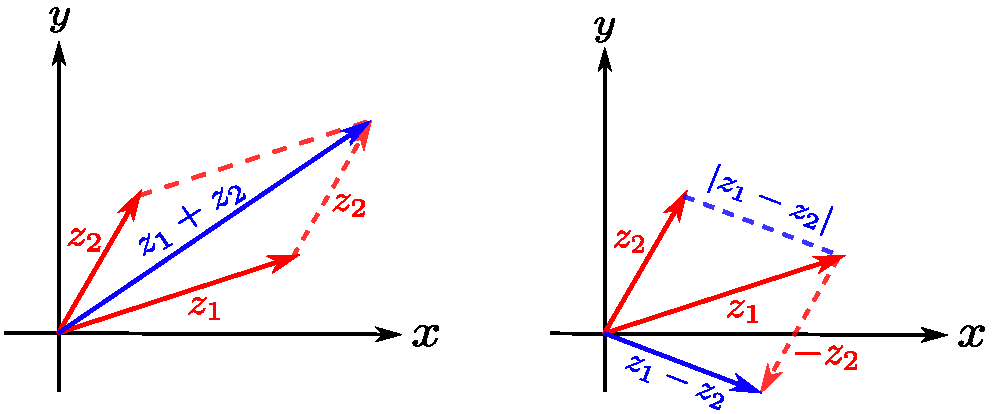
\includegraphics[scale=0.7]{Figuras/SumaCompejos.pdf}
    \caption{Interpretación geométrica de la suma y resta de números complejos.}
    \label{SumaComplejos}
\end{figure}

\begin{defi}
Para $z = x+iy \in \mathbb{C} $, definimos el \textbf{conjugado} de $z$ por el número
$$\bar{z} := x -iy.$$
\end{defi}

\textbf{Observación:} Geométricamente, $\bar{z}$ es la reflexión con respecto al eje $x$ del complejo $z$.

\begin{figure}[H]
    \centering
    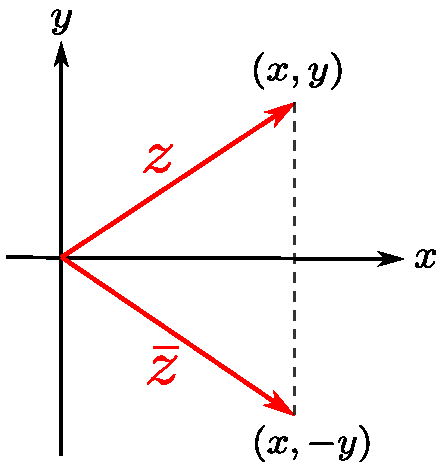
\includegraphics[scale=0.6]{Figuras/Conjugado.pdf}
    \caption{Gráfica del complejo conjugado.}
    \label{ComplejoConjugado}
\end{figure}

\begin{propo}\label{PropiedadesConjugadoModulo}
Si $z,z_1,z_2 \in \mathbb{C}$, entonces:

\begin{enumerate}
\item $$\overline{z_1 + z_2} = \overline{z_1} + \overline{z_2}; \quad \overline{z_1z_2} = \overline{z_1} \, \overline{z_2}; \quad \overline{\frac{z_1}{z_2}} = \frac{\overline{z_1}}{\overline{z_2}}, ~~ z_2 \neq 0.$$

\item $$z + \bar{z} \in \mathbb{R}; \quad \bar{\bar{z}} = z; \quad Re(z) = \frac{z + \bar{z}}{2};\quad Im(z)= \frac{z - \bar{z}}{2i}.$$

\item $$z \bar{z} = |z|^2; \quad |z| = |\bar{z}|; \quad \max\{|Re(z)|, |Im(z)|\} \leq |z|.$$

\item $$|z_1 z_2| = |z_1| \, |z_2|; \quad \left| \frac{z_1}{z_2} \right| = \frac{|z_1|}{|z_2|}, ~~ z_2 \neq 0.$$
\end{enumerate}

\end{propo}

\begin{proof}
Sean $z = x+iy$, $z_1 = x_1 + iy_1$ y $z_2 = x_2 + iy_2$ números complejos cualesquiera.

\begin{enumerate}
\item \begin{eqnarray*}
\overline{z_1 + z_2}  &=& \overline{(x_1+x_2) + i(y_1 + y_2)} \\\
&=&(x_1+x_2) - i(y_1 + y_2) \\
& =& (x_1 - iy_1) + (x_2 - iy_2) = \overline{z_1} + \overline{z_2}. \\
\overline{z_1 z_2} &=&  \overline{(x_1 x_2 - y_1y_2) + i(x_1y_2 + y_1x_2)} \\
&=&  (x_1 x_2 - y_1y_2) - i(x_1y_2 + y_1x_2) \\
&=& (x_1 -iy_1) (x_2 - iy_2) = \overline{z_1} \, \overline{z_2}.  \\
\overline{\frac{z_1}{z_2}} &=& \overline{z_1 z_2^{-1}} \\
&=& \overline{z_1} \, \overline{z_2^{-1}} \\
&=& \overline{z_1} \, \frac{x_2 - i(-y_2)}{x_2^2 + y_2^2} \\
&=& \overline{z_1} \, (\overline{z_2})^{-1} = \frac{\overline{z_1}}{\overline{z_2}}, ~~ z_2 \neq 0.
\end{eqnarray*}

\item \begin{eqnarray*}
z + \bar{z} &=& (x+iy) + (x-iy) = 2x \in \mathbb{R}. \\
\bar{\bar{z}} &=& \overline{x -iy} = x+iy = z. \\
Re(z) &=& \frac{(x+iy) + (x-iy)}{2} = \frac{z + \bar{z}}{2}. \\
Im(z) &=& \frac{(x+iy) - (x-iy)}{2i} = \frac{z - \bar{z}}{2i}.
\end{eqnarray*}

\item \begin{eqnarray*}
z \bar{z} &=& (x+iy)(x-iy) = x^2 + y^2 = |z|^2. \\
|z| &=& \sqrt{x^2+y^2} = \sqrt{x^2 + (-y_2)^2} = |\bar{z}|.
\end{eqnarray*}

Del cálculo III, sabemos que
$$|x| \leq \norm{(x,y)} ~~\mbox{y}~~ |y| \leq \norm{(x,y)}.$$

Como $Re(z) = x$ e $Im(z) = y$, se tiene que
$$\max\{|Re(z)|, |Im(z)|\} \leq \sqrt{x^2+y^2} = |z|.$$

\item 
\begin{equation*}
|z_1 z_2|^2 = (z_1 z_2) \, (\overline{z_1z_2}) = (z_1 \overline{z_1}) (z_2 \overline{z_2}) = |z_1|^2|z_2|^2 = (|z_1||z_2|)^2 ~\Rightarrow~ |z_1 z_2| = |z_1||z_2|.
\end{equation*}
\begin{equation*}
\left| \frac{z_1}{z_2} \right| = \left|z_1 z_2^{-1}\right| = |z_1| \, |z_2^{-1}| = |z_1| \, \left| \frac{x-iy}{x^2+y^2} \right| = |z_1| \, \frac{\sqrt{x^2+y^2}}{x^2+y^2} = |z_1| \,|z_2|^{-1} = \frac{|z_1|}{|z_2|}.
\end{equation*}

\end{enumerate}
\end{proof}

\begin{propo}[Desigualdad triangular]
Para cualquier par de números complejos $z_1$ y $z_2$, se tiene
$$|z_1 + z_2| \leq |z_1| + |z_2|.$$
\end{propo}

\begin{proof}
Utilizando las propiedades dadas en la proposición \ref{PropiedadesConjugadoModulo}, se tiene que
\begin{eqnarray*}
|z_1 + z_2|^2 &=& (z_1 + z_2) \overline{(z_1 + z_2)} \\
&=& (z_1 + z_2)(\overline{z_1} + \overline{z_2}) \\
&=& z_1 \overline{z_1} + z_1 \overline{z_2} + z_2 \overline{z_1} + z_2 \overline{z_2} \\
&=& |z_1|^2 + (z_1 \overline{z_2} + \overline{z_1 \overline{z_2}}) + |z_2|^2.
\end{eqnarray*}

Ahora, como $z_1 \overline{z_2} + \overline{z_1 \overline{z_2}}= 2 Re(z_1 \overline{z_2}) \leq 2 |z_1 \overline{z_2}| = 2 |z_1| \; |z_2|$, obtenemos que
$$|z_1 + z_2|^2 \leq |z_1|^2 + 2  |z_1| \; |z_2| + |z_2|^2 = (|z_1| + |z_2|)^2.$$

Por lo tanto,
$$|z_1 + z_2| \leq |z_1| + |z_2|.$$
\end{proof}

Por inducción, se puede demostrar que
\begin{corolario}
Si $z_1, z_2, \dots, z_n \in \mathbb{C}$, entonces
$$\left| \sum_{i=1}^n z_i \right| \leq \sum_{i=1}^n |z_i|.$$
\end{corolario}

\begin{corolario}
Si $z_1, z_2 \in \mathbb{C}$, entonces
$$||z_1| - |z_2|| \leq |z_1 + z_2|.$$
\end{corolario}

\begin{proof}
Sean $z_1, z_2 \in \mathbb{C}$ cualesquiera, se tiene que
\begin{equation}
|z_1| = |(z_1 + z_2) - z_2| \leq |z_1 + z_2| + |z_2| ~\Rightarrow~ |z_1| - |z_2| \leq |z_1 + z_2| \label{Desi.Trian1}
\end{equation}

y 
\begin{equation}
|z_2| = |(z_1 + z_2) - z_1| \leq |z_1 + z_2| + |z_1| ~\Rightarrow~ - |z_1 + z_2| \leq |z_1| - |z_2| \label{Desi.Trian2}.
\end{equation}

Combinando \eqref{Desi.Trian1} y \eqref{Desi.Trian2}, obtenemos
$$- |z_1 + z_2| \leq |z_1| - |z_2| \leq |z_1 + z_2| \Leftrightarrow ||z_1| - |z_2|| \leq |z_1 + z_2|.$$
\end{proof}

\section{Forma polar}

En coordenadas cartesianas, un complejo $z$ se identifica con un punto del plano de coordenadas $(x,y)$. Por otro lado, las coordenadas polares de este punto están dadas por las ecuaciones
\begin{eqnarray*}
x &=& r \cos \theta, \\
y &=& r \sin \theta .
\end{eqnarray*}

\begin{figure}[H]
    \centering
    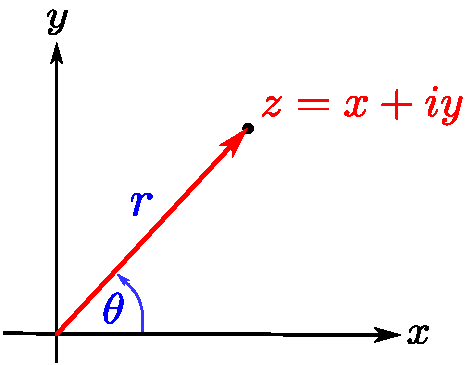
\includegraphics[scale=0.6]{Figuras/Polar.pdf}
    \caption{Coordenadas polares del complejo $z = x +iy$.}
    \label{Polares}
\end{figure}

donde $r$ es la longitud del segmento que une el origen con el punto $(x,y)$ y $\theta$ es la magnitud, en radianes, del ángulo que forma este segmento con la parte positiva del eje $x$.

Así,
$$z = x+iy = r \cos \theta + ir \sin \theta = r (\cos \theta + i \sin\theta).$$

A esta última expresión se le conoce como la \textbf{forma polar} del complejo $z$. 

El ángulo $\theta$ se llama \textbf{argumento} de $z$ y se denota por
$$\theta = \arg(z).$$

Notar que $r = |z|$ y que 
$$\tan \theta = \frac{y}{x}.$$

\textbf{Observación:} Si $z = 0$, $\theta$ está indefinido. De modo que cualquier número complejo que vaya ser escrito en polares se sobreentiende que es distinto de cero.

\begin{ejemplo}
 La forma polar del complejo $z = 1+i$ es
\begin{eqnarray*}
z &=& \sqrt{2} \left( \cos \frac{\pi}{4} + i \sin \frac{\pi}{4} \right) \\
&=& \sqrt{2} \left( \cos \left( -\frac{7\pi}{4}\right) + i \sin \left( - \frac{7\pi}{4} \right) \right).
\end{eqnarray*} 
\end{ejemplo}

De este ejemplo, se desprende que el $\arg(z)$ no es único.

En general, se tiene que
$$z = r [\cos (\theta + 2k\pi) + i \sin(\theta + 2k\pi)], \quad k \in \mathbb{Z},$$

donde $\theta$ es cualquier valor particular del argumento  de $z$.
\\

El \textbf{argumento principal} de $\arg(z)$, denotado $\Arg{z}$, se define como el único valor de $\arg(z)$ tal que $- \pi < \arg(z) \leq \pi$.

Luego, es conveniente definir el argumento de un número complejo como la función multievaluada
$$\arg(z) \equiv \Arg{z} + 2k \pi, \quad z \in \mathbb{Z},$$

es decir, $\arg(z)$ corresponde a un \underline{conjunto} de valores para un determinando $z \in \mathbb{C}$.
\\

En el caso del ejemplo anterior, el argumento principal de $1+i$ es $Arg(z) = \frac{\pi}{4}$.
\\

Ahora, si consideramos $z_1 = -1$ y $z_2 = i$, entonces $z_1 z_2 = -i$ y, en tal caso, tenemos
$$arg(z_1 z_2) = arg(-i) = \frac{3}{2}\pi = \pi + \frac{\pi}{2} = arg(z_1) + arg(z_2).$$

Pero,
$$Arg(z_1) = \pi; \quad Arg(z_2) = \frac{\pi}{2};\quad Arg(z_1z_2) = - \frac{\pi}{2}.$$

Lo que muestra que 
$$Arg(z_1z_2) \neq Arg(z_1) + Arg(z_2).$$

Sin embargo, para el argumento, se tiene la siguiente proposición.

\begin{propo}
Si $z_1, z_2 \in \mathbb{C}\setminus \{0\}$, entonces
\begin{equation}
arg(z_1z_2) = arg(z_1) + arg(z_2).\label{Producto.arg}
\end{equation}
\end{propo}

\begin{proof}
Supongamos que
\begin{equation}
z_1 = |z_1| [\cos ( \arg(z_1)) + i \sin( \arg(z_1))]; \quad z_2 = |z_2| [\cos( \arg(z_2)) + i \sin ( \arg(z_2))], \label{DosComplejos}
\end{equation}

donde 
\begin{align*}
    \arg(z_1) = \Arg{z_1} + 2 k_1 \pi = \theta_1 + 2 k_1 \pi  ; \quad k_1 \in \mathbb{Z}, \\
     \arg(z_2) = \Arg{z_2} + 2 k_2 \pi= \theta_2 + 2 k_2 \pi ; \quad k_2 \in \mathbb{Z}.
\end{align*}

Luego,
\begin{eqnarray*}
z_1 z_2 &=& |z_1| |z_2| [\cos ( \arg(z_1)) + i \sin( \arg(z_1))][\cos ( \arg(z_2)) + i \sin( \arg(z_2))] \\
&=& |z_1 z_2| (\cos \theta_1 + i \sin\theta_1)(\cos \theta_2 + i \sin \theta_2) \\
&=& |z_1 z_2| [(\cos \theta_1 \cos \theta_2 - \sin \theta_1 \sin\theta_2) + i(\sin\theta_1 \cos\theta_2 + \sin\theta_2 \cos \theta_1) ] \\
&=& |z_1 z_2| (\cos(\theta_1 + \theta_2) + i \sin(\theta_1 +  \theta_2)).
\end{eqnarray*}

Así,
$$\arg(z_1 z_2) = \theta_ 1 + \theta_2 + 2k_{12} \pi = \Arg{z_1} + \Arg{z_2} + 2k_{12} \pi, \quad k_{12} \in \mathbb{Z}.$$

Entonces, hemos establecido que 
\begin{align*}
    \arg(z_1) + \arg(z_2) &= \Arg{z_1} + \Arg{z_2} + 2 (k_1 + k_2)\pi, \\
    \arg(z_1 z_2) &= \Arg{z_1} + \Arg{z_2} + 2 k_{12}.
\end{align*}

Como $k_1$, $k_2$ y $k_{12}$ son enteros arbitrarios, $ \arg(z_1) + \arg(z_2)$ y $ \arg(z_1 z_2)$ coinciden como conjuntos.
\end{proof}

Geométricamente, el producto $z_1z_2$ en forma polar, se aprecia en la siguiente figura.

\begin{figure}[H]
    \centering
    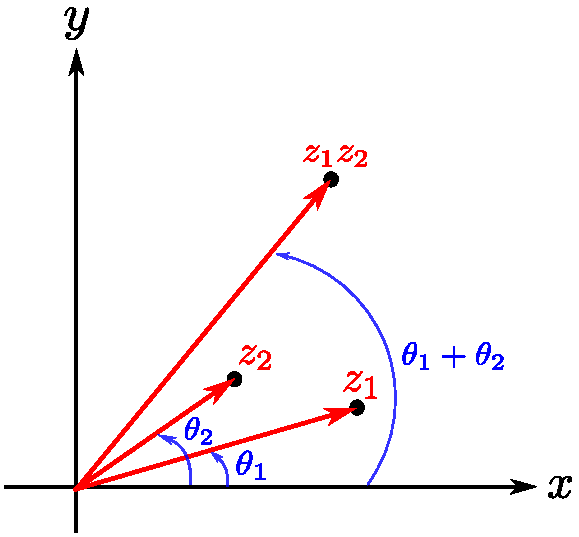
\includegraphics[scale=0.6]{Figuras/MultiplicacionComplejos.pdf}
    \caption{Interpretación geométrica del producto de números complejos en forma polar.}
    \label{ProductosComplejos}
\end{figure}

La ecuación 
$$z_1 z_2 = r_1r_2 (\cos(\theta_1 + \theta_2) + i \sin(\theta_1 +  \theta_2))$$

nos dice que la forma polar del único inverso multiplicativo de un número complejo no nulo
$$z = r (\cos \theta + i \sin \theta)$$

es
$$z^{-1} = \frac{1}{r} [\cos(-\theta) + i \sin(-\theta)],$$

siendo el producto de estas formas polares igual a la unidad.
\\

Como $\frac{z_1}{z_2} = z_1z_2^{-1}$, tenemos la siguiente expresión para el cociente de los dos números complejos no nulos \eqref{DosComplejos}:
$$\frac{z_1}{z_2} = \frac{r_1}{r_2} [\cos (\theta_1 - \theta_2) + i \sin(\theta_1- \theta_2)].$$

De la misma manera que el producto, ésto puede utilizarse para comprobar la afirmación
$$arg\left( \frac{z_1}{z_2} \right) = arg(z_1) - arg(z_2).$$
 
\section{Fórmula de Euler, potencias y raíces}

La ecuación
$$e^{i\theta} = \exp(i\theta) = \cos\theta + i \sin \theta$$

válida para todo $\theta \in \mathbb{R}$, se conoce como \textbf{fórmula de Euler}. 

Notemos que
$$e^{i \theta_1} e^{i \theta_2} = e^{i(\theta_1 + \theta_2)}$$

el cual corresponde al mismo tratamiento que conocemos del caso real. En particular,
$$e^{i\theta} e^{-i\theta} = 1,$$

es decir, $e^{- i\theta} = \frac{1}{e^{i\theta}}$ corresponde al inverso multiplicativo de $e^{i\theta}$.
\\

Si escribimos un número complejo no nulo en forma polar
$$z = r (\cos\theta + i \sin\theta),$$

la fórmula de Euler permite expresar $z$ más conveniente en \textbf{forma exponencial}:
$$z = r e^{i\theta}$$

y su inverso multiplicativo resulta ser
$$z^{-1} = \frac{1}{r} e^{-i\theta}.$$

Sean los complejos no nulos $z_1 = r_1 e^{i\theta_1}$ y $z_2 = r_2 e^{i\theta_2}$, se tiene que
\begin{eqnarray*}
z_1z_2 &=& r_1r_2 e^{i(\theta_1 + \theta_2)}. \\
\frac{z_1}{z_2} &=& \frac{r_1}{r_2} e^{i(\theta_1 - \theta_2)}.
\end{eqnarray*}

Es evidente que dos números complejos no nulos $z_1 = r_1 e^{i\theta_1}$ y $z_2 = r_2 e^{i\theta_2}$ son iguales si y sólo si $r_1 = r_2$ y $\theta_1 = \theta_2 + 2k\pi$, para algún $k \in \mathbb{Z}$.

\begin{teorema}
Sea $n \in \mathbb{Z}$ y sea $z= r (\cos \theta + i \sin \theta)$ un número complejo en forma polar. Entonces,
$$z^n = r^n (\cos (n\theta) + i\sin(n\theta)).$$
\end{teorema}

\begin{proof}
\
\\

\textbf{Caso 1:} Si $n > 0$, procederemos por inducción.

Para $n = 1$, es fácil de ver que el teorema se verifica.

Supongamos que para $n \in \mathbb{N}$ se satisface:
$$z^n = r^n (\cos(n\theta) + i \sin(n\theta).$$

Luego,
\begin{eqnarray*}
z^{n+1} = z^n z &=& [r^n (\cos (n\theta) + i\sin(n\theta))][r (\cos \theta + i \sin \theta)] \\
&=& r^{n+1} (\cos((n+1) \theta)) + i \sin((n+1) \theta))).
\end{eqnarray*}

Por lo tanto, el teorema es cierto para $n \in \mathbb{N}$.

\textbf{Caso 2:} Si $n = 0$, el convenio $z^0=1$ nos permite escribir: $z^0 = r^0 (\cos(0\cdot \theta) + i \sin(0 \cdot \theta)).$
\\

\textbf{Caso 3:} Si $n <0$, entonces
\begin{eqnarray*}
z^n = (z^{-1})^{-n} &=& r^n (\cos((-n)(-\theta)) + i \sin((-n)(-\theta))) \\
&=& r^n (\cos (n\theta) + i\sin(n\theta)).
\end{eqnarray*}

De esta manera, el teorema se verifica para todo $n \in \mathbb{Z}$.

\end{proof}

\textbf{Observación:} Equivalentemente, en forma exponencial, el teorema dice $(re^{i\theta})^n = r^n e^{in\theta}$. Si $r= 1$, obtenemos la \textbf{fórmula de De Moivre}:
$$(\cos \theta + i \sin\theta)^n = \cos(n \theta) + i \sin(n\theta).$$

\begin{defi}
Sea $n \in \mathbb{N}$. Dado un número complejo $z_0$, decimos que $z$ es una raíz $n$-ésima de $z_0$ si $z^n = z_0$.
\end{defi}

\begin{teorema}
Si $n \in \mathbb{N}$ y $z_0 \in \mathbb{C} \setminus \{0\}$ con forma polar $z_0 = r_0 (\cos \theta_0 + i \sin\theta_0) $, entonces $z_0$ tiene exactamente $n$ raíces $n$-ésimas distintas dadas por
$$\sqrt[n]{r_0} \left[ \cos \left( \frac{\theta_0 + 2k\pi}{n} \right) + i \sin \left( \frac{\theta_0 + 2k\pi}{n} \right)\right], \quad k = 0,1, \dots, n-1.$$
\end{teorema}

\begin{proof}
Las raíces $n$-ésimas de $z_0$ son los $z \in \mathbb{C}$ tales que
$$z^n = z_0.$$

Ésto implica que
$$|z^n| = |z|^n = |z_0|~\Rightarrow~ |z| = \sqrt[n]{|z_0|} = \sqrt[n]{r_0}.$$

Escribiendo $z$ en forma polar, $z = r (\cos \theta + i \sin \theta)$, obtenemos:
\begin{eqnarray}
[r (\cos \theta + i \sin \theta)]^n &=& r_0 (\cos \theta_0 + i \sin\theta_0)  \\
\Leftrightarrow ~ r^n (\cos (n\theta) + i \sin (n\theta)) &=& r_0 (\cos \theta_0 + i \sin\theta_0) \\
\Leftrightarrow \quad r^n \cos(n\theta) = r_0 \cos\theta_0  &\wedge & r^n \sin (n\theta)  = r_0 \sin \theta_0. \label{raíz}
\end{eqnarray}

Como $|z| = r = \sqrt[n]{r_0}$, la ecuación \eqref{raíz} nos queda
\begin{eqnarray}
\cos(n\theta) = \cos\theta_0  &\wedge &   \sin (n\theta)  =  \sin \theta_0 \\
\Rightarrow \qquad \qquad \qquad n \theta &=& \theta_0 + 2 m\pi, \quad m \in \mathbb{Z} \\
\Rightarrow  \qquad \qquad \qquad ~~ \theta &=& \frac{\theta_0}{n} + \frac{2 m \pi}{n}, \quad m \in \mathbb{Z}. \label{raiz2}
\end{eqnarray}

Ahora, por el algoritmo de la división, la división de los enteros $m/n$ nos dice que existen $q \in \mathbb{Z}$ (cociente) y $0\leq k < n$ (resto) tales que
$$m = n q + k.$$

Reemplazando en \eqref{raiz2}:
$$\theta = \frac{\theta_0}{n} + \frac{2 (nq + k) \pi}{n} = \frac{\theta_0 + 2k\pi}{n} + 2q\pi.$$

Luego,
$$z = \sqrt[n]{r_0}  \left[ \cos \left( \frac{\theta_0 + 2k\pi}{n} + 2q\pi \right) + i \sin \left( \frac{\theta_0 + 2k\pi}{n} + 2q\pi\right)\right].$$

Por lo tanto, por periocidad de las funciones seno y coseno, se obtienen $n$ raíces $n$-ésimas para $z_0$ dadas por
$$\sqrt[n]{r_0} \left[ \cos \left( \frac{\theta_0 + 2k\pi}{n} \right) + i \sin \left( \frac{\theta_0 + 2k\pi}{n} \right)\right], \quad k = 0,1, \dots, n-1.$$

Para demostrar que estas $n$ raíces son distintas, supongamos que para $0 \leq j,l \leq n-1$ se tiene
$$\frac{\theta_0 + 2j\pi}{n} = \frac{\theta_0 + 2l\pi}{n}.$$
 
Es claro entonces que $j = l$ y por tanto los valores de $\theta$ son diferentes cuando $j\neq l$ y $0 \leq j,l \leq n-1$.

\end{proof}

\begin{defi}
Llamamos \textbf{raíces n-ésimas de la unidad} a las raíces $n$-ésimas de 1, visto como número complejo.
\end{defi}

Si $z_0 = 1 = (\cos(0) + i \sin (0))$, tenemos que las raíces de la unidad son
$$\cos \left( \frac{2k\pi}{n} \right) + i \sin \left( \frac{2k\pi}{n} \right), \quad k = 0,1, \dots, n-1.$$

Si  llamamos \cite{Churchill}
$$\omega_n = \cos \left( \frac{2\pi}{n} \right) + i \sin \left( \frac{2\pi}{n} \right),$$

entonces el conjunto de las raíces $n$-ésimas de la unidad es
$$\{1, \omega_n, \omega_n^2, \dots, \omega_n^{n-1}\}.$$

\begin{propo}
Algunas propiedades de las raíces de la unidad se enuncian a continuación:

\begin{itemize}
\item[(i)] El producto entre raíces $n$-ésimas de la unidad es una raíz $n$-ésima de la unidad.

\item[(ii)] Si $c$ es una raíz $n$-ésima de $z_0$, entonces el conjunto de todas las raíces $n$-ésimas de $z_0$ se puede expresar como 
$$z_0^{1/n} = \left\{ c \, \omega_n^k : k = 0, 1, \dots, n-1 \right\}.$$

\item[(iii)] La suma de las raíces $n$-ésimas de la unidad es cero.
\end{itemize}
\end{propo}

\begin{proof}
Sean $\omega_n^i$ y $\omega_n^j$ dos raíces $n$-ésimas de la unidad, ésto es,
$$(\omega_n^i)^n = 1 ~~\mbox{y}~~ (\omega_n^j)^n = 1.$$

Notemos que
$$(\omega_n^i \omega_n^j)^n = (\omega_n^i)^n (\omega_n^j)^n = 1. $$

De esta manera, hemos probado el ítem $(i)$.

Si escribimos $z_0$ en forma polar, $z_0 =  r_0 (\cos \theta_0 + i \sin\theta_0)$, entonces
$$c = \sqrt[n]{r_0} \left[ \cos \left( \frac{\theta_0 + 2k\pi}{n} \right) + i \sin \left( \frac{\theta_0 + 2k\pi}{n} \right)\right] $$

para algún $k \in \{0,1,\dots,n-1\}$ fijo.

Como las demás raíces de $z_0$ tienen el mismo módulo de $c$ pero con un argumento aumentado en $\frac{2\pi}{n}$, el conjunto de las raíces $n$-ésimas de $z_0$ es  
$$z_0^{1/n} = \left\{ c \, \omega_n^k : k = 0, 1, \dots, n-1 \right\}.$$

Probando así el ítem $(ii)$.
\\

Queda como ejercicio para el lector probar que para $z \in \mathbb{C} \setminus\{1\}$, se obtiene que 
$$1 + z + z^2 + \cdots + z^n = \frac{1 -z^{n+1}}{1 - z}.$$

Como $\omega_n \neq 1$, obtenemos
$$1 + \omega_n + \omega_n^2 + \cdots + \omega_n^{n-1} = \frac{1 -  \omega_n^n}{1 - \omega_n} = \frac{1-1}{1-\omega_n} = 0.$$

Probando así, el ítem $(iii)$.

\end{proof}

\textbf{Observaciones:}

\begin{enumerate}
\item A partir de la proposición anterior, el conjunto $ \{1, \omega_n, \omega_n^2, \dots, \omega_n^{n-1}\}$ forma un subgrupo de $\mathbb{C}$.

\item Geométricamente, las raíces de la unidad están ubicadas en la circunferencia unitaria del plano y distribuidas como los vértices de un polígono regular inscrito en la circunferencia unitaria (ver figura \ref{RaizUno}).

\begin{figure}[H]
    \centering
    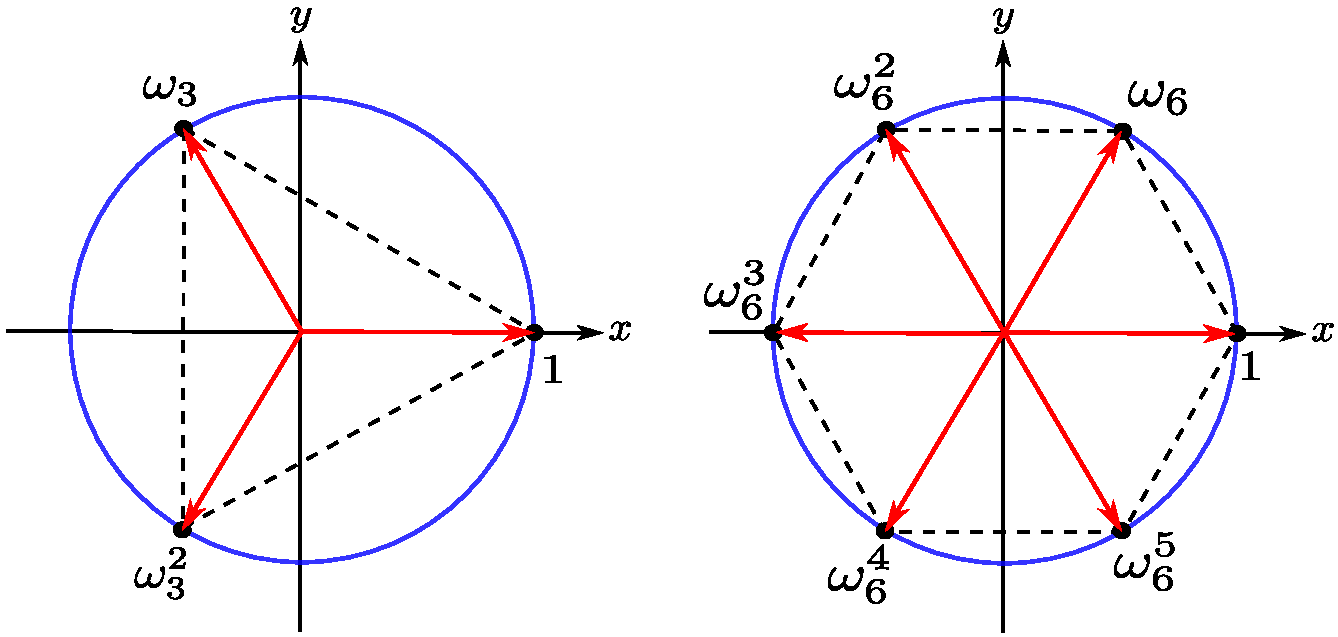
\includegraphics[scale=0.5]{Figuras/RaizUnidad.pdf}
    \caption{Raíces $n$-ésima de la unidad para $n = 3$ y $n = 6$.}
    \label{RaizUno}
\end{figure}

\end{enumerate}

\section{Topología de los números complejos}

 Recordemos que si $z \in \mathbb{C}$, entonces el módulo de $z$ satisface las siguientes propiedades:

\begin{enumerate}
\item $|z| \geq 0$.

\item $ |z| = 0 ~\Leftrightarrow~ z = 0$.

\item Si $z_1, z_2 \in \mathbb{C}$, entonces $|z_1 z_2| = |z_1|\, |z_2|$.

\item Si $z_1, z_2 \in \mathbb{C}$, entonces $|z_1 + z_2| \leq |z_1| + |z_2|$.
\end{enumerate}

Utilizando el módulo, se define la siguiente función
$$d: \mathbb{C} \times \mathbb{C} \longrightarrow \mathbb{R}, \quad (z_1,z_2) \mapsto d(z_1,z_2) = |z_1 - z_2|.$$

Para $z_1, z_2, z_3 \in \mathbb{C}$, notemos que $d$ satisface:

\begin{itemize}
\item[D1.] $d(z_1,z_2) \geq 0$.

\item[D2.] $d(z_1,z_2) = 0 ~\Leftrightarrow~ z_1 = z_2$.

\item[D3.] $d(z_1,z_2) = d(z_2, z_1)$.

\item[D4.] $d(z_1,z_3) \leq d(z_1,z_2) + d(z_2,z_3)$.
\end{itemize}

Por las propiedades satisfechas por la función $d$, ésta se llama \textbf{distancia o métrica} en $\mathbb{C}$, implicando que el par $(\mathbb{C},d)$ es un \textbf{espacio métrico}.

\begin{defi}
Sea $z_0 \in \mathbb{C}$ fijo y sea $\varepsilon >0$ un número real dado. El conjunto
$$B(z_0, \varepsilon) = \{z \in \mathbb{C} ~:~ d(z,z_0) = |z-z_0| < \varepsilon\}$$

se llama \textbf{bola abierta o vecindad o disco abierto de centro $z_0$ y radio $\varepsilon$}.
\end{defi}

Notemos que $B(z_0, \varepsilon)$ corresponde al lugar geométrico de un círculo de centro $z_0$ y radio $\varepsilon$ que no contiene su circunferencia.

\begin{figure}[H]
    \centering
    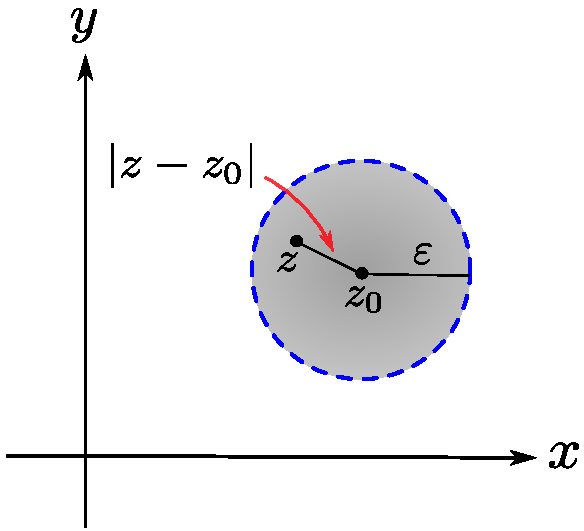
\includegraphics[scale=0.55]{Figuras/BolaAbierta.pdf}
    \caption{Bola abierta de centro $z_0$ y radio $\varepsilon$ en el plano complejo.}
    \label{BolaAbierta}
\end{figure}

\begin{defi}
Sea $A$ un subconjunto de $\mathbb{C}$ y sea $z \in \mathbb{C}$. Diremos que $z$ es un \textbf{punto interior de $A$} si 
$$\exists \varepsilon >0 :~ B(z,\varepsilon) \subseteq A.$$

Notar que, en este caso, $z \in A.$
\end{defi}

\begin{defi}
Un subconjunto $A$ en $\mathbb{C}$ se llama \textbf{conjunto abierto} si todos sus puntos son puntos interiores de $A$, en otras palabras, si
$$(\forall z \in A)(\exists \varepsilon(z) >0)(B(z, \varepsilon(z)) \subseteq A).$$
\end{defi}

\begin{defi}
Sea $A$ un subconjunto de $\mathbb{C}$ y sea $z \in \mathbb{C}$. Diremos que $z$ es un \textbf{punto exterior de $A$} si
$$\exists \varepsilon >0 :~ B(z,\varepsilon) \cap A = \emptyset.$$

Notar que, en este caso, $z \notin A$.
\end{defi}

\begin{defi}
Sea $A$ un subconjunto de $\mathbb{C}$ y sea $z \in \mathbb{C}$. Diremos que $z$ es un \textbf{punto de frontera de $A$} si $z$ no es punto interior y tampoco punto exterior de $A$. El conjunto de todos los puntos frontera de $A$ se llama \textbf{frontera de $A$} y se denota por $Fr(A)$. 
\end{defi}

\begin{ejemplo}
El conjunto $\{z \in \mathbb{C} : |z| = 1\}$ es la frontera de: $\{z \in \mathbb{C} : |z|<1\}$ y $\{z \in \mathbb{C} : |z|\leq 1\}$.
\end{ejemplo}

\begin{defi}
Un subconjunto $F$ de $\mathbb{C}$ se llama \textbf{conjunto  cerrado} si su complemento $F^c = \mathbb{C} \setminus F$ es abierto.
\end{defi}

\begin{defi}
Sea $S$ un subconjunto de $\mathbb{C}$, se llama \textbf{clausura o adherencia de $S$} al conjunto $S \cup Fr(S)$ y se denota por $\overline{S}$.
\end{defi}

\textbf{Observación:} Existen conjuntos que no son ni abiertos ni cerrados, por ejemplo, $\{z \in \mathbb{C} : 0 < |z| \leq 1\}$. En cambio, el conjunto de los números complejos es abierto y cerrado a la vez.

\begin{defi}
Un subconjunto $S$ de $\mathbb{C}$ se llama \textbf{conjunto conexo} si cualquier par de puntos $z_1, z_2 \in S$ puede unirse por un camino poligonal consistente de un número finito de segmentos unidos por sus punto iniciales y finales y que se encuentra enteramente contenido en $S$. 
\end{defi}

\begin{ejemplo}
Algunos ejemplos de conjuntos conexos son: $\{z \in \mathbb{C} : |z| <1\}$; $\{z \in \mathbb{C} : |z| \leq 1\}$; $\{z \in \mathbb{C} : 1 < |z| <2 \}$, ver figura \ref{Conexo}.

\begin{figure}[H]
    \centering
    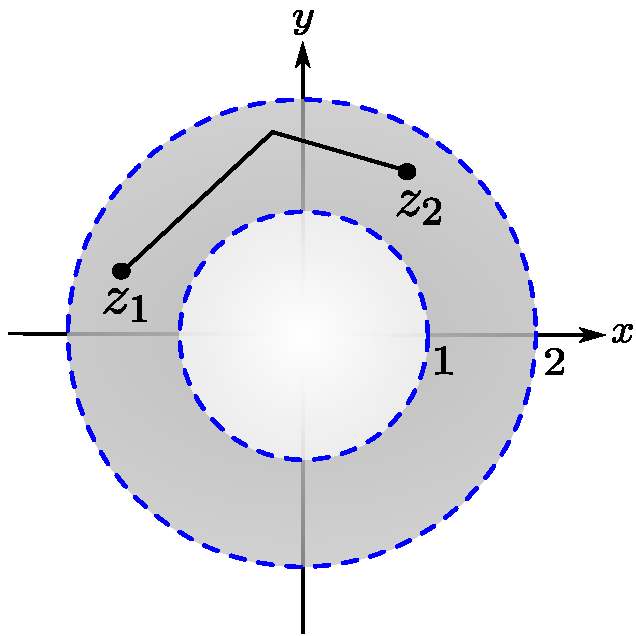
\includegraphics[scale=0.45]{Figuras/EjemploConexo.pdf}
    \caption{Gráfica del conjunto conexo $\{z \in \mathbb{C} : 1 < |z| <2 \}$.}
    \label{Conexo}
\end{figure}

\end{ejemplo}

\begin{defi}
Un conjunto conexo abierto se llama \textbf{dominio} y un dominio con alguna o ninguna o toda su frontera se llama \textbf{región}.
\end{defi}

\textbf{Observación:} Note que cualquier vecindad es un dominio.

\begin{defi}
Un subconjunto $S$ de $\mathbb{C}$ se llama \textbf{conjunto acotado} si existe $M >0$ tal que

$$(\forall z \in S)(|z| \leq M).$$

En caso contrario, se llamará conjunto no acotado.
\end{defi}

\begin{ejemplo}
El primer cuadrante del plano, una recta, el complemento de cualquier vecindad, etc, son ejemplos de conjuntos no acotados.
\end{ejemplo}

\begin{defi}
Sea $A$ un subconjunto de $\mathbb{C}$ y sea $z_0 \in \mathbb{C}$. Diremos que $z_0$ es un \textbf{punto de acumulación de $A$} si

$$(\forall \varepsilon > 0)([B(z_0, \varepsilon) \setminus \{z_0\} ]\cap A \neq \emptyset).$$ 
\end{defi}

\section{El punto al infinito}

A menudo es conveniente considerar, junto con el plano complejo, un punto especial llamado \textbf{punto al infinito} y que lo denotaremos por $\infty$. Para visualizar este punto, consideraremos una esfera unitaria $S$ centrada en el origen del sistema rectangular $xyz$ elegido para el espacio $\mathbb{R}^3$ y asumamos que el plano complejo es el plano $xy$ que pasa a través del ecuador.

\begin{figure}[H]
    \centering
    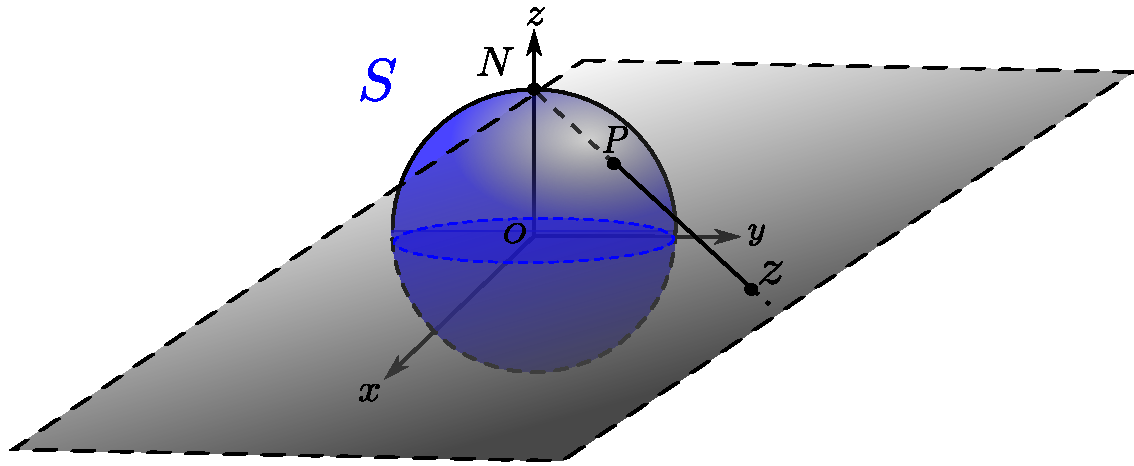
\includegraphics[scale=0.5]{Figuras/EsferaRiemann.pdf}
    \caption{Esfera de Riemann.}
    \label{EsferaRiemann}
\end{figure}

Observar que la recta en el espacio, que pasa por el punto $N = (0,0,1)$ (polo norte de la esfera) y un punto $z$ dado en el punto complejo, determina un único punto $P$ de la esfera. De igual manera, la recta que pasa por el polo norte y un punto dado $P$ en la esfera, determina un único punto $z$ del plano complejo. En otras palabras, existe una aplicación biyectiva
$$f: S - \{N\} \longrightarrow \mathbb{C}, \quad P \mapsto z.$$

Ahora, si al plano complejo le agregamos un elemento, que lo denotaremos por el símbolo $\infty$, el nuevo conjunto $C \cup \{\infty\} = \overline{\mathbb{C}}$ lo llamamos \textbf{plano extendido}. De esta manera, la aplicación $f$ puede extenderse también a $N$ de la siguiente forma:
$$f: S  \longrightarrow \mathbb{C}, \quad P \mapsto \left\{ \begin{array}{ccl}
z &,& P \neq N \\
\infty &,& P = N
\end{array} \right. .$$

Este proceso de correspondencia se llama \textbf{proyección estereográfica} y la esfera es conocida por \textbf{esfera de Riemann}.

Con el fin de extender la adición y multiplicación en el plano complejo al plano extendido, definiremos las siguientes reglas:
\begin{eqnarray*}
z + \infty = \infty &;& z \cdot \infty = \infty,  ~ z \neq 0\\
\infty + \infty = \infty &;& \infty \cdot \infty = \infty.
\end{eqnarray*}

Observar que la imagen del hemisferio norte menos su polo de la esfera de Riemann corresponde al exterior de la bola unitaria y recíprocamente. Además, para un pequeño número positivo $\varepsilon$, aquellos puntos del plano complejo exteriores a la circunferencia $|z| = \frac{1}{\varepsilon}$  corresponden a puntos de la esfera próximos a $N$. Llamaremos al conjunto $B(\infty, \frac{1}{\varepsilon}) = \{z \in \mathbb{C} : |z| > \frac{1}{\varepsilon}\}$ un \textbf{entorno de $\infty$}.